\chapter{Transforming our Communities}


\begin{figure}[h]
	\centering
	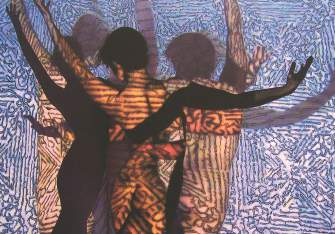
\includegraphics[height=12cm]{TeX_files/4-0.png}
	\caption{Artysta: Anastasia Keck}
	\label{2-0}
\end{figure}

\noindent\textcolor{ProcessBlue}{\textbf{\LARGE{Jak możemy rozpocząć przeciwdziałanie opresji w naszych społecznościach?}}}\\

Możemy zacząć od rozmowy o tym. Jest wiele zalet, które wynikają z rozmowy o opresji w naszych społecznościach. Między innymi:

\begin{checkboxlist}
	\item Jeśli rozumiesz i uznajesz to, co naprawdę się dzieje, możesz przeciwdziałać temu bezpośrednio i zacząć efetkywnie rozwiązywać problem. Nierówność nie ma żadnych zalet, jedynie koszty.
	\item Musimy dostrzegać wszystkie sposoby, na jakie ludzie są ranieni przez opresję, ponieważ dzięki temu mogą oni zacząć mówić prawdę o tym, jak opresywne jest nasze społeczeństwo i miejmy nadzieję, doporwadzić do pozytywnych zmian.
	\item Ludzie wiedzieliby, że nie są sami.
	\item Jeśli tego nie odkrywamy, pozostawiamy to władzom, a ich perspektywa jest ważna, ale ograniczona. Jeśli to odkrywamy, mamy rzeczywistą szansę, by zmniejszyć rozmiar szaleństwa i opresji oraz doskonalić się osobiście i wspólnotowo.
	\item Aby można było jej przeciwdziałać, opresja musi być zrozumiana. W przypadku społeczności społeczość jako całośc musi rozumieć, jak opresja jest tworzona przez grupy i kierowana przeciwko indywidualnym członkom społeczności.
	\item Rozmawianie o tych problemach w bezpieczny sposób może mieć jedynie pozytywny efekt dla wszystkich.
	\item To może nam pomóc budować więzi: możemy uczyć się większej głębi o tym, jak wspierać osoby, które są prowokowane przez emocję lub zachowania ingerujące w ich życie.
	\item Odkrywanie opresji mogłoby dać więcej współczucia. Ludzie mają skłonność to odczłowieczania tego, czego nie rozumieją.
	\item Społeczność odniesie korzyści, ponieważ stanie się bardziej świadoma włansego cierpienia i być może wyjdzie z cienia, by dołaczyć do programów lub stworzyć nowe, tak by opresja stała się pustym wyrazem.
	\item Eksponowanie opresji pomaga jednostkom uzyskać poczucie sprawiedliwości oraz pomaga społeczności dostrzegać opresję i ją zatrzymywać.
\end{checkboxlist}

\noindent\textcolor{ProcessBlue}{\textbf{\LARGE{Jak możesz zacząć przeciwdziałać opresji w twojej społeczności?}}}\\

\noindent\rule{\textwidth}{1pt}\\
\noindent\rule{\textwidth}{1pt}\\
\noindent\rule{\textwidth}{1pt}\\
\noindent\rule{\textwidth}{1pt}\\
\noindent\rule{\textwidth}{1pt}\\
\noindent\rule{\textwidth}{1pt}\\
\noindent\rule{\textwidth}{1pt}\\
\noindent\rule{\textwidth}{1pt}\\\\



\begin{figure}[h]
	\centering
	
\includegraphics[height=12cm]{TeX_files/4-1.png}
	\caption{Artysta: Till Krech}
	\label{2-0}
\end{figure}

\noindent\textcolor{ProcessBlue}{\textbf{\LARGE	{Kroki, które możemy podjąć, by złagodzić opresję, to:}}}\\

\begin{multicols}{2}
	\begin{checkboxlist}
		\item Wykonaj pracę. Kształć się. Ludzie muszą się uczyć, mówić głośniej, być w porządku z uczuciem niewygody
		\item Dołącz do działań na rzecz społeczeństwa. Przyczyniaj się we własny sposób, niezależnie czy będzie to maszerowanie na ulicach, czy wypełnianie kopert
		\item Podpisuj petycje
		\item Przemawiaj na spotkaniach Rady Miasta
		\item Edukuj swoje dzieci
		\item Zakończ ciszę. Mów o tym. Nazywaj to. Okaż wsparcie
		\item Zwiększaj świadomość: rozmawiaj z przyjaciółmi
		\item Bądź szczery
		\item Mierz się z ‘izmami’ gdy się pojawiają
		\item Bądź dobrym sprzymierzeńcem
		\item Pomagaj pokazywać swojej społeczności, że jesteśmy tutaj
		\item Ucz dzieci, że bezdomni mają uczucia, oraz że rodzice LGBT są tacy sami jak inni rodzice
		\item Ludzie mogliby uczyć się o PTSD oraz rozumieć, że jest to częścią tego, kim jestem, docenialiby mnie oraz innych cierpiących
		\item Zapobiegaj znęcaniu się
		\item Działajcie razem oraz planujcie działanie w grupach. Grupy mogą kształcić się na temat opresji, przywilejów, rasizmu, kompetencji kulturowych i innych
		\item Wspieraj rodziny w swojej społeczności. Twórz międzypokoleniowe instytucje, uwzględniając dzieci i starszych
		\item Żądaj by bezdomni mieli pozowlenie, by spać w przytułkach. Mogliby budować system wsparcia dla aktywistów, by walczyć z opresją i wspierać ich wysiłki, ich głos oraz zmagania
		\item Wierzę, że pierwszym krokiem jest doskonalenie otwartego umysłu, by wierzyć, że wszyscy jesteśmy zdolni, by uzdrawiać i zmieniać
		\item Bierz udział w kampaniach pisania listów do firm i narzekaj
		\item Zaakceptuj, że istnieją ludzie tacy jak ty oraz, że chcesz im pomagać
		\item Zaakceptuj, że możesz tworzyć sztukę i poezję, ponieważ twoje życie jest podróżą
		\item Chódź na wiece i marsze by wpierać innych
		\item Podpisuj petycje i wysyłaj e-maile do polityków
		\item Przyklejaj anty-rasistowskie naklejki
		\item Rozmawiaj z innymi by zwiększać świadomość
		\item Stwórz wewnętrzny spokój, który jest niezniszczalny
	\end{checkboxlist}
\end{multicols}

\noindent\textcolor{ProcessBlue}{\textbf{\LARGE{Kroki, które już podjęliśmy, by złagodzić opresję, to:}}}\\

\begin{multicols}{2}
	\begin{checkboxlist}
		\item Już teraz mam pragnienie zmiany sytuacji oraz wprowadzenia innych w światło rozumienia, że życie jest piękne i wartościowe
		\item Wierzę, że uczucia związane z opresją dały mi ogromne współczucie i zrozumienie
		\item Pisałem i reżyserowałem krótkie przedstawienia oraz rysowałem i malowałem urocze obrazki. Nie mógłbym robić tych rzeczy, jeśli nie czułbym takiego bólu
		\item To sprawiło, że jestem silniejszy w swojej wierze
		\item Znalazlem przyjaciół oraz pogłębiłem relacje z innymi
		\item Wypowiadałem się
		\item Tworzyłem ziny
		\item Pomagałem tworzyć lub brałem udział w kilku ruchach przeciwko opresji
		\item Czasami myślę o tym, jak wiele ludzi może czuć się podobnie do mnie i to inspiruje mnie, by tworzyć ziny lub fikcję, mając na uwadzę, że może istnieć nieznana mi publiczność, która może odnaleźć wartość w moich słowach
		\item Odnalazłem akceptację w społeczności, która docenia ludzi za to kim są
		\item Odnalazłem poczucie wyzwolenia, kiedy zacząłem całkowicie się akceptować
		\item Staram się zaangażować innych użytkowników/ocalałych w tworzenie społeczności, która skupia się na alternatywnych ujęciach zdrowia psychicznego i dobrego samopoczucia oraz na politycznym działaniu, które ma przynieść systematyczną zmianę
		\item Jedynym "lekarstwem" na bezsilność jest społeczny i polityczny aktywizm - moim jedynym zastrzeżeniem jest potrzeba dbania o tych, którzy się wypalili i nie mogą odnaleźć przyjaznej społeczności. To jest rzecz, nad którą musimy pracować jako społeczność
		\item Nauczyłem się jak wzmocnić moje czaakry i moją aurę, tak aby nie być bombardowanym negatywną energią innych ludzi
		\item Traktuję priorytetowo moje własnej zdrowie, bezpieczeństwo oraz możliwość wyrażania siebie
		\item Staram się być dobry dla innych, aby robić wszystko, co mogę, jako osoba, aby czynić świat bardziej tolerancyjnym
		\item Odczuwam silną potrzebę, aby to wszystko zmienić, albo przynajmniej namieszać w tym wszystkim wielką łyżką
		\item Staram się filozofować w zaciszu sypialni, spacerować na zewnątrz, oraz pisać poezję, aby oddać sprawiedliwość takim uczuciom i nie ulec całkowitemu wypaleniu
		\item Organizuje się, aby budować siłę z naszymi ludźmi, aby przezwyciężyć naszą opresję
	\end{checkboxlist}
\end{multicols}

\noindent\textcolor{ProcessBlue}{\textbf{\LARGE{Jakie masz inne pomysły, by zmieniać swoją społeczność?}}}\\

\noindent\rule{\textwidth}{1pt}\\
\noindent\rule{\textwidth}{1pt}\\
\noindent\rule{\textwidth}{1pt}\\
\noindent\rule{\textwidth}{1pt}\\
\noindent\rule{\textwidth}{1pt}\\
\noindent\rule{\textwidth}{1pt}\\
\noindent\rule{\textwidth}{1pt}\\
\noindent\rule{\textwidth}{1pt}\\\\